% The study's challenges
%% The importance of energy and energy storage
En 2019, la consommation mondiale d'énergie finale a doublé par rapport à 1973 et a dépassé la barre des \qty{400}{\exa \joule}, dont \qty{19.7}{\percent} d'électricité \cite{birol_key_nodate}.\\
Les énergies renouvelables sont une des solutions pour répondre à cette demande croissante d'électricité tout en respectant l'environnement. Cependant, les périodes de production ne coïncidant pas nécessairement avec les périodes de consommation -- le cycle diurne étant un exemple -- il est nécessaire de pouvoir stocker efficacement l'énergie produite en attendant qu'elle soit consommée.

%% Presenting the SCs
Les supercondensateurs sont une bonne piste pour le stockage d'énergie. Ils sont composés d'électrodes de carbone poreuses séparées par une membrane perméable et plongées dans un électrolyte. Ceci permet le déplacement des charges d'une électrode à l'autre lorsque l'appareil est en charge ou en décharge (\autoref{fig:schema_supercondensateur}).\\
Ils se situent entre les batteries et les condensateurs en termes de densité d'énergie et de puissance, ainsi leur utilisation est répandue pour les véhicules électriques, systèmes d'alimentation sans fil ou encore appareils portables.

\begin{figure}[hb]
    \centering
    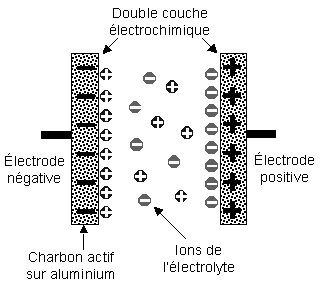
\includegraphics[height=5cm]{supercondensateur.png}
    \caption{Schéma d'un supercondensateur}
    \label{fig:schema_supercondensateur}
\end{figure}

% Presenting the state of the art
Plusieurs études ayant des sujets connexes ont déjà été réalisées : la densité relative d'ions de l'électrolyte et le potentiel peuvent être ciblés pour étudier la structure de la Double Couche Électrique (EDL)\cite{jiang_molecular_2016}, ou encore la densité d'ions et de charges pour étudier l'adsorption des ions à l'interface électrode/électrolyte\cite{cole_ion_2011}. Cependant, nous voulons adopter une approche légèrement différente : en utilisant un potentiel réactif pour les interactions entre les particules [\reaxff{}] plutôt que des modèles rigides (ex: SPC/E, TIP3P, etc.), mettre en place la polarisation du système en contrôlant directement le voltage entre les électrodes [\echemdid{}] plutôt qu'en modifiant manuellement les charges des atomes des électrodes, et en essayant d'ajouter des défauts aux électrodes (atome manquant, atome ajouté à la surface).

% Presenting the problem
Malgré son importance, la complexité de la structure de ces électrodes est trop grande pour l'étude que nous avons envisagée, notamment à cause de leur porosité, de la présence de réseaux de pores et de défauts\cite{bo_design_2018}. Ainsi, nous avons choisi d'étudier un système modèle pour nous concentrer sur l'observation des mécanismes de base de ces appareils, comme l'adsorption des ions et la formation de la Double Couche Électrique (EDL). En faisant cela, nous espérons pouvoir mieux comprendre le fonctionnement des supercondensateurs.

% Presenting the plan
Dans un premier temps, nous présentons ce système modèle : ses caractéristiques, sa construction et sa mise en place.
Puis, nous discutons des outils que nous utilisons dans nos simulations, à savoir le potentiel réactif \reaxff{}\cite{van_duin_reaxff_2001}\cite{russo_atomistic-scale_2011}\cite{senftle_reaxff_2016}, la mise en place de la polarisation du système à l'aide d'\echemdid{}\cite{onofrio_voltage_2015}, et leur implémentation au sein de \lammps{}.
Enfin, nous présentons les résultats obtenus et observations faites lors de cette étude, notamment par rapport à l'adsorption des ions à la surface des électrodes, l'influence de leurs défauts, et la répartition des charges en leur sein.
